\documentclass{article}
\usepackage[T1]{fontenc}
\usepackage[polish]{babel}
\usepackage[utf8]{inputenc}
\usepackage{amsmath}
\usepackage{amssymb}
\usepackage{graphicx}

\title{Potencjał grawitacyjny - MES}
\author{Wojciech Dąbek}
\date{Styczeń 2024}

\begin{document}

\maketitle

\section{Problem}

\begin{gather*}
    \frac{d^2 \Phi}{dx^2} = 4 \pi G \rho(x)\\
    \Phi(0) = 5\\
    \Phi(3) = 4\\
    \rho(x) =
    \begin{cases}
        0 & \text{dla } x \in [0,1]\\
        1 & \text{dla } x \in (1,2]\\
        0 & \text{dla } x \in (2,3]
    \end{cases}
\end{gather*}
Szukam funkcji \textit{$\Phi$} spełniającej powyższe warunki.

\section{Wyprowadzenie sformułowania wariacyjnego}

\[\Phi''(x) = 4 \pi G \rho(x)\]
Wprowadzam funkcję testującą \(v: [0,3] \to \mathbb{R},\ v \in V\), gdzie \textit{V} przyjmuję jako przestrzeń funkcji zerujących się na brzegach.
Obustronnie mnożę przez \textit{v} i całkuję na \([0,3]\).
\[\int_0^3 \Phi'' v\ dx = 4 \pi G \int_0^3 \rho v\ dx\]
Całkuję przez części, aby pozbyć się drugiej pochodnej.
\[[\Phi' v]_0^3 - \int_0^3 \Phi' v'\ dx = 4 \pi G \int_0^3 \rho v\ dx\]
Skoro \(v \in V \Leftrightarrow v(0) = v(3) = 0\), to \([\Phi' v]_0^3 = 0\). Mam więc:
\[-\int_0^3 \Phi' v'\ dx = 4 \pi G \int_0^3 \rho v\ dx\]
Wprowadzam oznaczenia:
\begin{gather*}
    B(\Phi, v) = -\int_0^3 \Phi' v'\ dx\\
    L(v) = 4 \pi G \int_0^3 \rho v\ dx = 4 \pi G \int_1^2 v\ dx
\end{gather*}
Gdzie \(B(\Phi, v)\) jest funkcjonałem biliniowym, a \(L(v)\) jest funkcjonałem liniowym.\\
Równanie można więc zapisać jako:
\[B(\Phi, v) = L(v)\]

\section{Rozszerzenie warunków brzegowych}

Ze względu na niezerowe warunki Dirichleta, konstruuję przesunięcie:
\begin{gather*}
    \Phi = w + \tilde{\Phi}\\
    w \in V\\
    \tilde{\Phi}(x) = 5 - \frac{x}{3}
\end{gather*}
Tak przyjęta funkcja \(\tilde{\Phi}\) spełnia warunki brzegowe, tzn. \(\tilde{\Phi}(0) = 5, \tilde{\Phi}(3) = 4\).\\
Można zatem wrócić do równania i zapisać je jako:
\[B(w + \tilde{\Phi}, v) = L(v)\]
Korzystając z liniowości \textit{B} względem pierwszego argumentu:
\[B(w, v) = L(v) - B(\tilde{\Phi}, v)\]
Przyjmując \(\tilde{L}(v) = L(v) - B(\tilde{\Phi}, v)\) można ostatecznie zapisać:
\[B(w, v) = \tilde{L}(v)\]

\section{Konstrukcja podprzestrzeni\\\textit{N} elementów skończonych \(V_h \subset V\)}

W celu skonstruowania podprzestrzeni \(V_h \subset V\) dzielę zbiór \([0, 3]\) na \textit{N} równych części o długości \(h = \frac{3}{N}\).\\
Punkty brzegowe takiego podziału to więc:
\begin{gather*}
    x_0 = 0,\ x_k = kh,\ x_N = 3\\
    x_{k-1} = x_k - h,\ x_{k+1} = x_k + h
\end{gather*}

\noindent
Wybieram funkcje bazowe postaci:
\begin{align*}
    &e_k(x) =
    \begin{cases}
        \frac{x - x_{k-1}}{h} = \frac{x}{h} - k + 1 \text{ dla } x \in [x_{k-1}, x_k]\\
        \frac{x_{k+1} - x}{h} = k + 1 - \frac{x}{h} \text{ dla } x \in (x_k, x_{k+1}]\\
        0 \text{ w przeciwnym przypadku}
    \end{cases} \text{dla } k = 1, 2, \ldots, N-1\\
    &e'_k(x) =
    \begin{cases}
        \frac{1}{h} \text{ dla } x \in [x_{k-1}, x_k]\\
        -\frac{1}{h} \text{ dla } x \in (x_k, x_{k+1}]\\
        0 \text{ w przeciwnym przypadku}
    \end{cases}
\end{align*}

\noindent
Mogę więc zdefiniować \(V_h = \langle e_1, \ldots, e_{N-1} \rangle\) (generowaną przez funkcje \(e_k\)).

\section{Problem przybliżony w przestrzeni \(V_h\)}

Z rozważanego wyżej problemu oryginalnego przechodzę na\\
problem przybliżony: Znaleźć \(w_h \in V_h\) spełniające
\begin{gather*}
    \forall v_h \in V_h : B(w_h, v_h) = \tilde{L}(v_h)\\
    w \approx w_h = \sum_{i=1}^{N-1} w_i e_i
\end{gather*}

\noindent
Mam więc układ \(N-1\) równań:
\[B \left(\sum_{i=1}^{N-1} w_i e_i, v_j \right) = \tilde{L}(v_j) \text{ dla } j = 0,\ 1,\ 2,\ \ldots,\ N\]
Przyjmuję \(v_j = e_j\).
\[B \left(\sum_{i=1}^{N-1} w_i e_i, e_j \right) = \tilde{L}(e_j)\]
Korzystając z liniowości \textit{B} względem pierwszego argumentu:
\[\sum_{i=1}^{N-1} w_i B(e_i, e_j) = \tilde{L}(e_j)\]
Zapisuję ten układ równań w postaci macierzowej:
\begin{gather*}
    \begin{bmatrix}
        B(e_1, e_1) & B(e_2, e_1) & \cdots & B(e_{N-1}, e_1)\\
        B(e_1, e_2) & B(e_2, e_2) & \cdots & B(e_{N-1}, e_2)\\
        \vdots & \vdots & \ddots & \vdots\\
        B(e_1, e_{N-1}) & B(e_{N-1}, e_{N-1}) & \cdots & B(e_{N-1}, e_{N-1})
    \end{bmatrix}
    \begin{bmatrix}
        w_1 \\ w_2 \\ \vdots \\ w_{N-1}
    \end{bmatrix}
    =
    \begin{bmatrix}
        \tilde{L}(e_1) \\ \tilde{L}(e_2) \\ \vdots \\ \tilde{L}(e_{N-1})
    \end{bmatrix}
\end{gather*}
\noindent
Mam więc takie wartości elementów tych macierzy:
\begin{gather*}
    B(e_i, e_j) = -\int_0^3 e'_i e'_j\ dx\\
    \tilde{L}(e_j) = L(e_j) - B(\tilde{\Phi}, e_j)\\
    L(e_j) = 4 \pi G \int_1^2 e_j dx
\end{gather*}

\noindent
Jak łatwo zauważyć, \(B(e_i, e_j) = 0\) zawsze, gdy \(j < i-1 \text{ lub } j > i+1\).\\
W przeciwnym wypadku:
\begin{gather*}
    B(e_i, e_{i+1}) = B(e_{i+1}, e_i) = -\int_{x_i}^{x_{i+1}} e'_i e'_{i+1}\ dx\\
    B(e_i, e_i) = -\int_{x_{i-1}}^{x_{i+1}} e'_i e'_i\ dx \text{ dla } i=1,2,\ldots,N-1
\end{gather*}

\noindent
Podobnie \(L(e_j) = 0\) zawsze, gdy \(hj < 1 \text{ lub } hj > 2\).\\
W przeciwnym wypadku:
\[L(e_j) = 4 \pi G \int_{x_{j-1}}^{x_{j+1}} e_j\ dx \text{ dla } j=1,2,\ldots,N-1\]
Pozostało do rozważenia: \(\left(\text{wiedząc, że } \tilde{\Phi}' = -\frac{1}{3}\right)\)
\[B(\tilde{\Phi}, e_j) = \frac{1}{3} \int_{x_{j-1}}^{x_{j+1}} e'_j\ dx \text{ dla } j=1,2,\ldots,N-1\]

Aby zastosować kwadraturę Gaussa-Legendre'a do przybliżenia wartości całek muszę zamienić przedziały całkowania na \([-1,1]\). Można to zrobić tak:
\[\int_a^b f(x)dx = \int_{-1}^1 f\left(\frac{b-a}{2} t + \frac{a+b}{2}\right)\frac{b-a}{2}\ dt\]
Stosując zasadę
\[\int_{-1}^1 f(x)dx \approx \sum_{i=1}^n w_i f(x_i)\]
Otrzymuję dla przedziału \([a,b]\):
\[\int_a^b f(x)dx \approx \frac{b-a}{2} \sum_{i=1}^n w_i f\left(\frac{b-a}{2} t_i + \frac{a + b}{2}\right)\]
Przyjmuję \(n=2\), więc \(w_i = 1 \text{ i } t_i = \pm \frac{1}{\sqrt{3}}\)
\[\int_a^b f(x)dx \approx \frac{b-a}{2} \left[f\left(\frac{b-a}{2} \cdot \frac{1}{\sqrt{3}} + \frac{a+b}{2}\right) + f\left(\frac{a-b}{2} \cdot \frac{1}{\sqrt{3}} + \frac{a+b}{2}\right)\right]\]

\vspace{5mm}
\noindent
Pozostaje obliczyć te wartości i rozwiązać układ równań, w czym pomoże mi dołączony program napisany w języku R.

\vspace{5mm}
\noindent
Przy znalezionych \(w_0, w_1, \ldots, w_N\) ostatecznym rozwiązaniem jest:
\[\Phi(x) = w + \tilde{\Phi} \approx \sum_{i=0}^N w_i e_i + 5 - \frac{x}{3}\]

\begin{figure}[h]
    \centering
    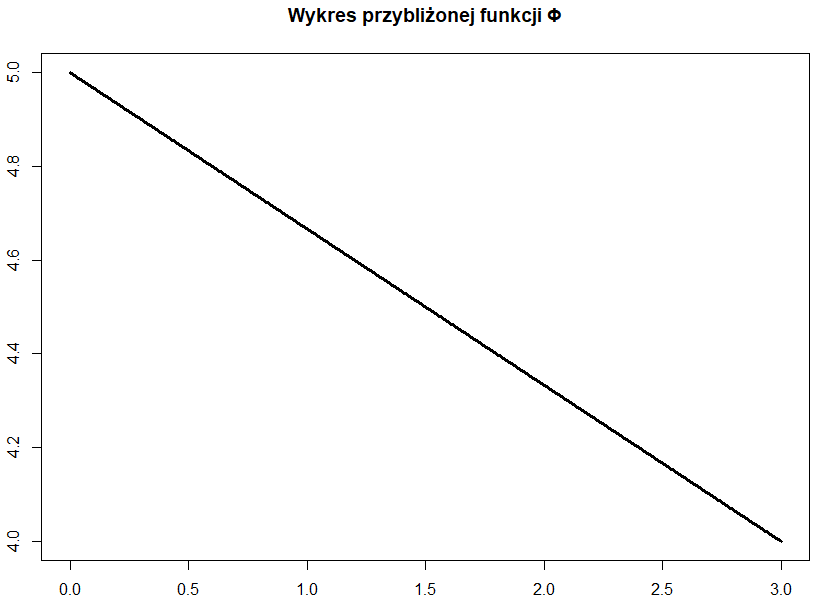
\includegraphics[width=1\linewidth]{graph1.png}
    \caption{Wyrysowany wykres dla \(N=20\)}
    \label{fig:graph1}
\end{figure}

\newpage
\noindent
Duży wpływ na kształt wykresu ma bardzo mała wartość \(G \approx 6.6743 \cdot 10^{-11}\).\\
Gdybym w jej miejsce przyjął wartość \(6.6743 \cdot 10^{-2}\) otrzymałbym:

\begin{figure}[h]
    \centering
    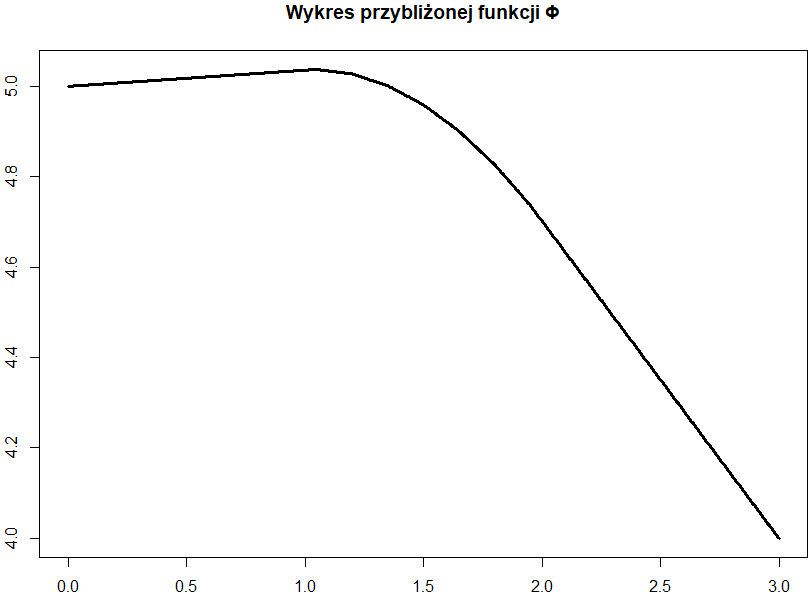
\includegraphics[width=1\linewidth]{graph2.png}
    \caption{Wyrysowany wykres dla \(G=6.6743 \cdot 10^{-2},\ N=20\)}
    \label{fig:graph2}
\end{figure}

\noindent
Widać więc, że nie jest to funkcja liniowa.

\end{document}
